% Source - https://tex.stackexchange.com/a/514356
% Posted by nidhin, modified by community. See post 'Timeline' for change history
% Retrieved 2026-07-02, License - CC BY-SA 4.0
% https://www.overleaf.com/learn/latex/CircuiTikz_package

\documentclass[border=5mm]{standalone}
\usepackage{tikz}
\usepackage[american,siunitx]{circuitikz}
\usetikzlibrary{arrows,shapes,calc, positioning, patterns, decorations, decorations.markings,quotes}
\tikzset{rotarrow/.pic={
\draw[thin,->] (-0.2,-0.2)  to [out=-60,in=60, looseness=4] ++(0,0.4) node [above=1mm] {\tikzpictext};
},
}

\begin{document}
    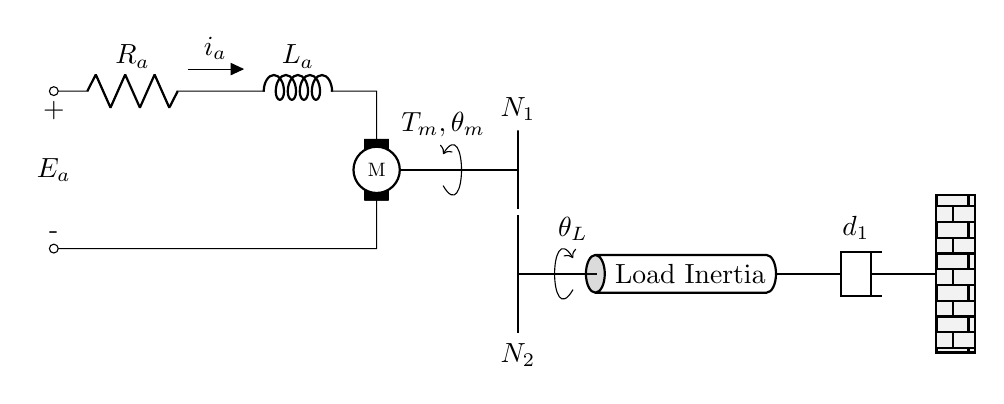
\begin{tikzpicture}[damper/.style={thick,
            decorate,
            decoration={markings,  
                mark connection node=dmp,
                mark=at position 0.5 with 
                {
                    \node (dmp) [thick, inner sep=0pt, 
                    transform shape, 
                    rotate=-90, 
                    minimum width=15pt, 
                    minimum height=10pt, draw=none] {};
                    \draw [thick] ($(dmp.north east)+(4pt,0)$) -- 
                    (dmp.south east) -- (dmp.south west) -- 
                    ($(dmp.north west)+(4pt,0)$);
                    \draw [thick] ($(dmp.north)+(0,-8pt)$) -- 
                    ($(dmp.north)+(0,8pt)$);
        }}},]

        \draw (0,2) to[R=$R_a$,o-] ++(2,0) to[short,f=$i_a$] ++(0.1,0) to[L,cute inductor, l=$L_a$,]  ++(2,0)  to[short,  name=M1] ++(0,-2) to[short,-o] (0,0);
        \draw (M1) node[elmech,scale=0.7](M2){M};
        \path (0,2)node[below]{+} -- node[midway]{$E_a$} (0,0)node[above]{-};
        \draw[thick] (M2.east) -- pic[pic text={$T_m,\theta_m$}]{rotarrow} ++(1.5,0) -- +(0,0.5) node [anchor=south] {$N_1$} -- +(0,-0.5) coordinate (N1);

        \draw[thick] ([yshift=-2]N1) -- ++(0,-1.5) node [below] {$N_2$} ++(0,0.75) --  pic[xscale=-1,pic text={$\theta_L$}]{rotarrow} ++(1,0) node [cylinder, black, shape border rotate=180, draw,
        minimum height=2, minimum width=1, aspect=0.5,cylinder uses custom fill, cylinder end fill = black!70,anchor=west,xshift=-0.15cm, fill opacity=0.2,text opacity=1] (c) {Load Inertia};
        \draw [damper] (c.east) -- node[above=3mm] {$d_1$} ++(0:2)   node[draw, rectangle, minimum height=2cm, minimum width =0.5cm,anchor=west,preaction={fill=gray!10},pattern=north east lines,pattern=bricks]{};
    \end{tikzpicture}
\end{document}
